\documentclass[12pt]{article}
\usepackage{setspace}
\setlength{\parindent}{4em}
\usepackage{fancyvrb}
\usepackage{graphicx}
\usepackage{geometry}
\renewcommand\thesection{\arabic{section}}
\renewcommand\thesubsection{\thesection.\arabic{subsection}}
\geometry{letterpaper, portrait, margin=1in}

%%%Title Page%%%
\title{\vspace{3cm}Lab 07\bigbreak Toy Processor with Memory on the Basys2 Board}
\author{
{\normalsize
\begin{tabular}{l r r}
 & \textbf{Ryan Cruz} & \textbf{Zachary Davis}\\
\textbf{Category} & ryan.cruz25@uga.edu & zachdav@uga.edu\\
\hline
Pre-lab 						  & 50 & 50\\
In-lab Module \& Testbench Design & 50 & 50\\
In-lab Testbench Sim. \& Analysis & 50 & 50\\
In-lab FPGA Synthesis \& Analysis & 50 & 50\\
Lab Report Writing 				  & 50 & 50\\
\end{tabular}
}}
%%%%%%%%%%%%%%%%%

\begin{document}
\maketitle
\newpage
\setstretch{2.5} % for custom spacing
\tableofcontents
\setstretch{1} % for custom spacing
\newpage

\section{Lab Purpose} \vspace{-.7cm} \line(1,0){470}
	\paragraph{}
		With the design of the toy processor complete, we can now implement it physically. With some tweaks to make it compatible, we can put it on the Basys2 board and load some simple programs onto it. 
		
\section{Implementation Details} \vspace{-.7cm} \line(1,0){470}
		
		
	\subsection{Part 1 - Clock and Bypass Circuits}

	\textbf{Clock}\\
	The clock for the processor, when implemented on the board, will be provided by the board. 
	This clock is too fast for human reading, so we will generate a push button clock and step through each operation.

		 \begin{figure}[h]
		 	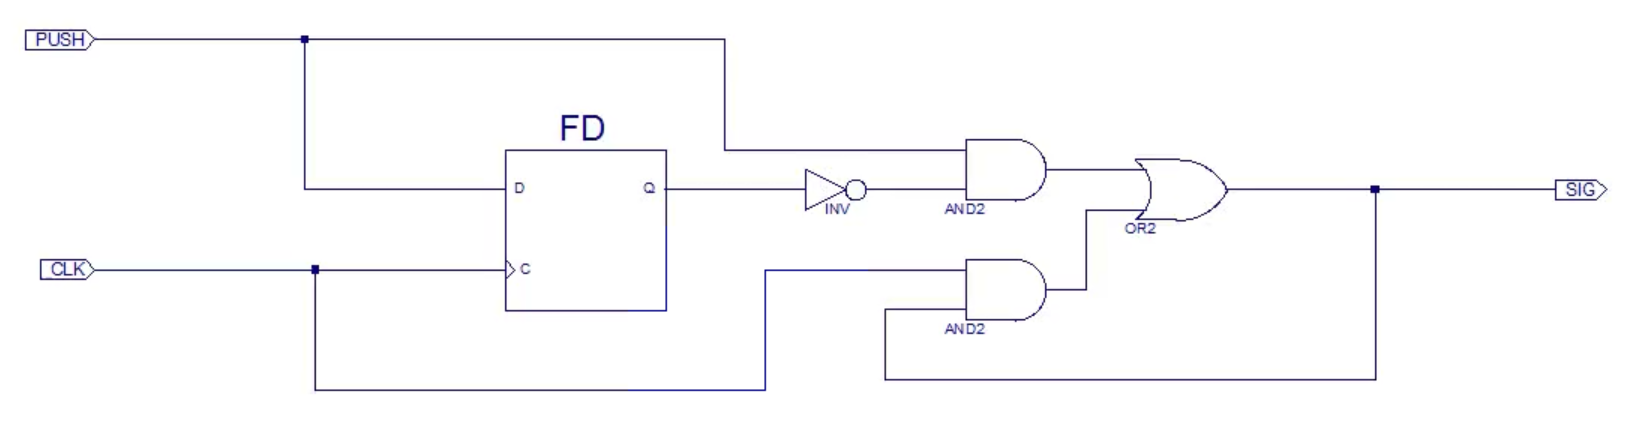
\includegraphics[scale=.55]{clk_signal_sch.PNG}
		 	\caption{Design of the clock signal created in Xilinx. (Designed on paper but just turned in a print out of this for prelab)}
		 \end{figure}

		
		\begin{Verbatim}[frame=single, fontsize= \small]
//Clock Testbench
`timescale 1ns/1ps

module clk_signal_tb;

	reg CLK = 1'b0;
	reg PUSH = 1'b0;

	wire SIG;

	initial // Clock process for CLK
		begin
			forever
			begin
				CLK = 1'b0;
				#100; 
				CLK = 1'b1;
				#100;
			end
		end
	
	clk_signal_sch UUT (
		.CLK(CLK),
		.PUSH(PUSH),
		.SIG(SIG));

	initial 
		begin

			#285;
			PUSH = 1'b1;
			#200;
			PUSH = 1'b0;
			#400;
			PUSH = 1'b1;
			#600;
			PUSH = 1'b0;

		end
endmodule

		\end{Verbatim}
		The test bench simply simulates button presses, and covers the test case of a holding the button as well. Results of the waveform are shown in the Expirimental Results section.\\\newline\textbf{Bypass}\\
		To avoid having to press the button 256 times to transition states, we designed a bypass so that the clock is automatic. 
		 \begin{figure}[h]
		 	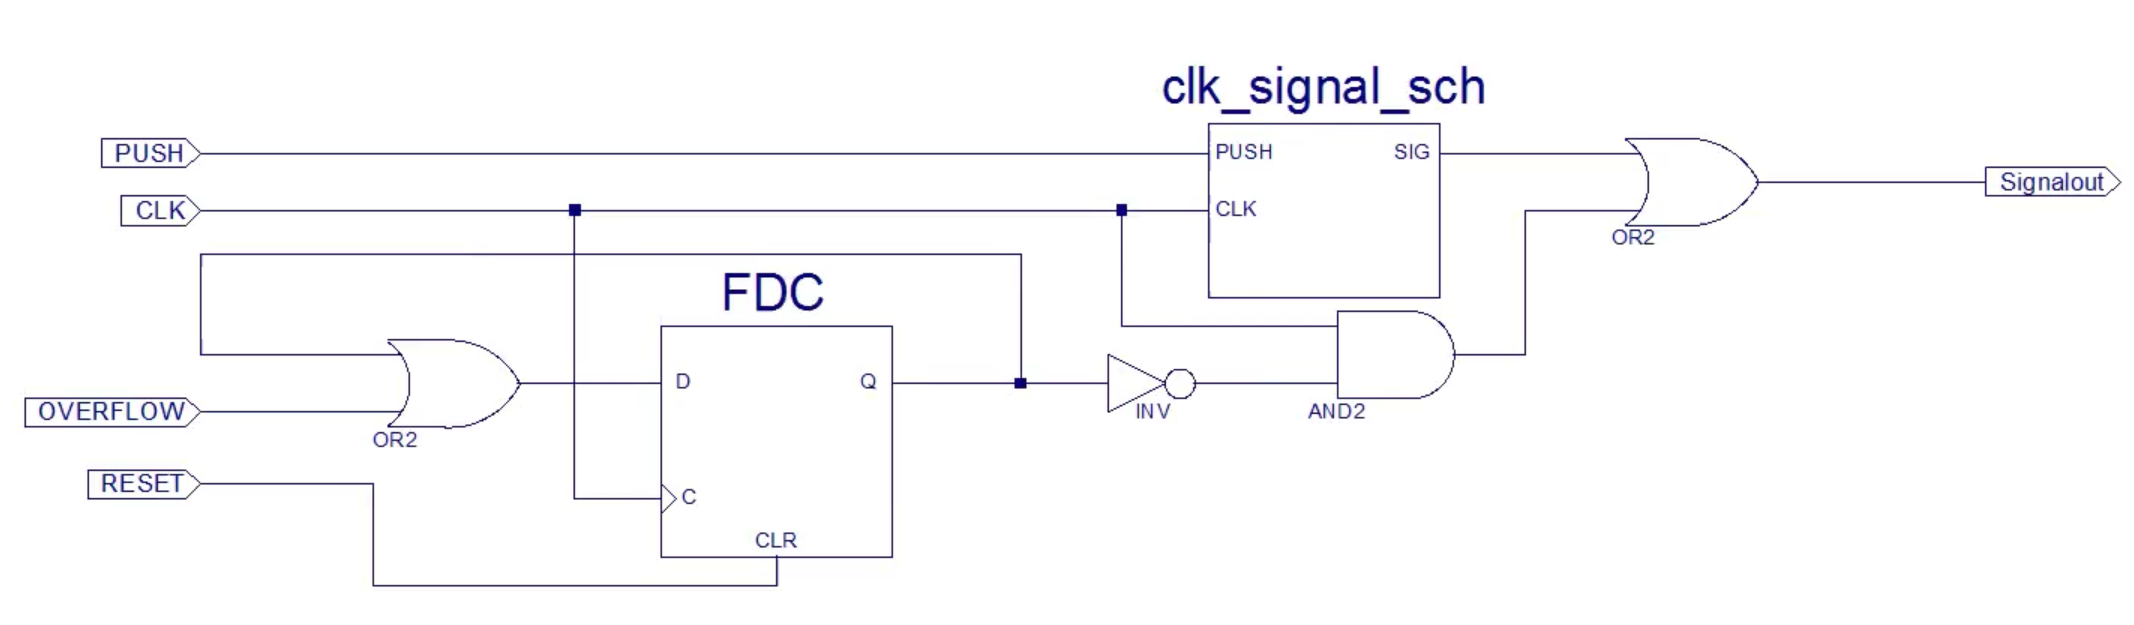
\includegraphics[scale=.45]{BypassClk.PNG}
		 	\caption{Design of the bypass clock signal created in Xilinx. (Designed on paper but just turned in a print out of this for prelab)}
		 \end{figure}
\begin{Verbatim}[frame=single, fontsize= \small]
`timescale 1ns/1ps

module BypassClk_tb;

	reg CLK = 1'b0;
	reg OVERFLOW = 1'b0;
	reg PUSH = 1'b0;
	reg RESET = 1'b0;
	
	wire Signalout;

	initial // Clock process for CLK
		begin
			forever
			begin
				CLK = 1'b0;
				#50; 
				CLK = 1'b1;
				#50;
			end
		end

	BypassClk UUT (
		.CLK(CLK),
		.OVERFLOW(OVERFLOW),
		.PUSH(PUSH),
		.RESET(RESET),
		.Signalout(Signalout));

	initial 
		begin
			// ------------- Current Time: 140ns
			#140;
			RESET = 1'b1;
			// -------------------------------------

			// ------------- Current Time: 340ns
			#200;
			RESET = 1'b0;
			// -------------------------------------
			
			// ------------- Current Time: 440ns
			#100;
			PUSH = 1'b1;
			// -------------------------------------

			// ------------- Current Time: 640ns
			#200;
			PUSH = 1'b0;
			// -------------------------------------

			// ------------- Current Time: 740ns
			#100;
			PUSH = 1'b1;
			// -------------------------------------

			// ------------- Current Time: 840ns
			#100;
			PUSH = 1'b0;
			// -------------------------------------

			// ------------- Current Time: 940ns
			#100;
			OVERFLOW = 1'b1;
			// -------------------------------------

			// ------------- Current Time: 1040ns
			#100;
			OVERFLOW = 1'b0;
			// -------------------------------------

			// ------------- Current Time: 2140ns
			#200;
			PUSH = 1'b1;
			// -------------------------------------

			// ------------- Current Time: 2340ns
			#200;
			PUSH = 1'b0;
			#100;
			PUSH = 1'b1;
			#100;
			PUSH = 1'b0;
			// -------------------------------------
		end
endmodule
\end{Verbatim}


		\newpage
		\subsection{Part 2 - Programming the Basys2 Board}
		To make the processor compatible with the board and for it to be testable, we must program the seven segment display, similar to how we have done in previous labs. It will display the instructions, as well as the accumulator.

		 \begin{figure}[h]
		 	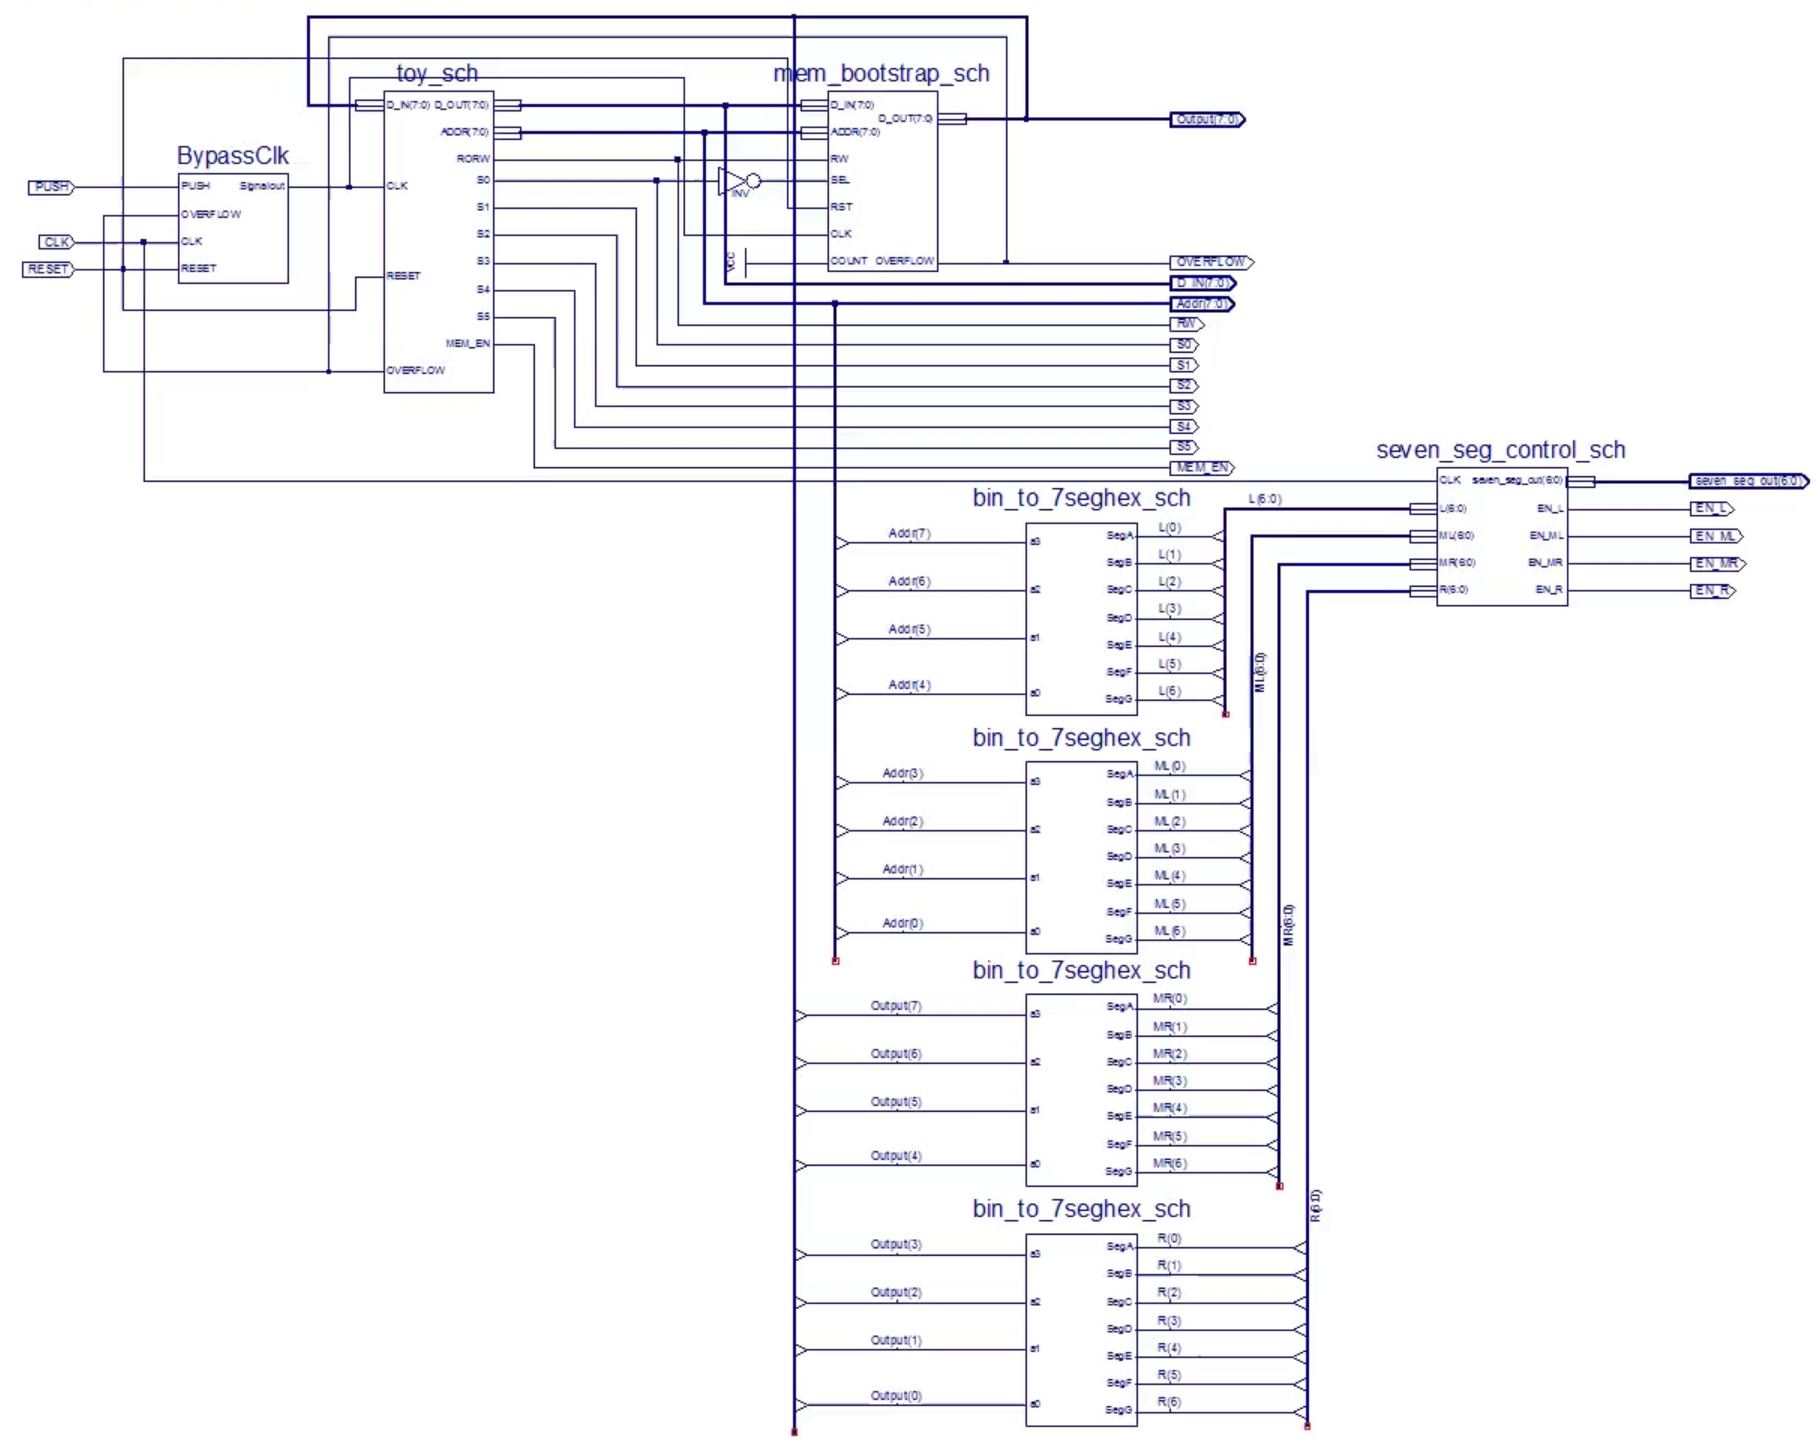
\includegraphics[scale=.5]{toyProcessor_Overall.PNG}
		 	\caption{Modifications to the ToyProcessorOverall schematic to add the seven segment displays.}
		 \end{figure}
\newpage

With the board ready for programs, we can now enter machinecode into ROM and actually see its output on the seven segment display. We will design two programs, with the 2nd testing all of the capabilities of our ToyProcessor.\\

The first program that we will load onto the board simply sums the numbers from 1-9 using the ADD instruction and then stores that sum. This program is not self-modifying, does not loop, and is linear -- it ends after the first run.
\begin{center}
\textbf{First Serial Addition Program}\\
\begin{tabular}{|l|l|l|}
\hline
Address & Instruction & Description\\
\hline
0       & 100	&CLR    \\
1       & 1		&ADD    \\
2       & 1		&1      \\
3       & 1		&ADD    \\
4       & 10	&2      \\
5       & 1		&ADD    \\
6       & 11	&3      \\
7       & 1		&ADD    \\
8       & 100	&4      \\
9       & 1		&ADD    \\
10      & 101	&5      \\
11      & 1		&ADD    \\
12      & 110	&6      \\
13      & 1		&ADD    \\
14      & 111	&7      \\
15      & 1		&ADD    \\
16      & 1000	&8      \\
17      & 1		&ADD    \\
18      & 1001	&9      \\
19      & 10000	&STORE 	\\
20      & 45	&45		\\
\hline
\end{tabular}
\end{center}

\newpage
This program stricly speaking does the exact same thing as the program above. This program summs the values from 0 - 9 and stores the answer. The difference of the program from the other is that it is entirly self-modifying, includes basic branching, and the use of all the instructions that we programmed for the CPU. We begin by clearing/soft-reset. We than add 10 and subtract 1 and then store the value. We do this rather than add 9 so that we can simply loop through the above portion and run though all the number from 9 to 0. If we started with 9 we would only get 8 to 0. Once we store the value we branch back to the add unless it is zero. This will add 8 then 7 then 6 and so on and so forth. Finally we store the resulting value.
\begin{center}
\textbf{Second Serial Addition Program}\\
\begin{tabular}{|l|l|l|}
\hline
Address & Instruction & Description \\
\hline
0       & 100	&CLR       \\
1       & 1		&ADD           \\
2       & 1010	&10        \\
3       & 10	&SUB         \\
4       & 1		&1          \\
5       & 10000	&STORE       \\
6       & 10	&2          \\
7       & 1000	&BNZ        \\
8       & 10010	&18       \\
9       & 1 	&ADD          \\
10      & 0		&0           \\
11      & 10000	&STORE       \\
12      & 1010	&10        \\
13      & 10000	&STORE       \\
14      & 1100100	&100     \\
15      & 100	&CLR         \\
16      & 1000	&BNZ        \\
17      & 1   	&1        \\
\hline
\end{tabular}
\end{center}

\subsection{UCF File}
	\begin{Verbatim}[frame=single, fontsize= \small]
######################################################################
###                Toy Proceesor Overall UCF File                  ###
######################################################################

NET s0 LOC=M5;        # LED 0 (on high)
NET s1 LOC=M11;       # LED 1 (on high)
NET s2 LOC=P7;        # LED 2 (on high)
NET s3 LOC=P6;        # LED 3 (on high)
NET s4 LOC=N5;        # LED 4 (on high)
NET s5 LOC=N4;        # LED 5 (on high)
NET MEM_EN LOC=P4;    # LED 6 (on high)
NET Overflow LOC=G1;  # LED 7 (on high)

### BASYS2 7-Segment LED:
NET EN_L LOC=K14;   # Left Digit (on low)
NET EN_ML LOC=M13;  # Middle Left Digit (on low)
NET EN_MR LOC=J12;  # Middle Right Digit (on low)
NET EN_R LOC=F12;   # Right Digit (on low)

### BASYS2 7-Segment Segments:
NET seven_seg_out<0> LOC=L14;  # LED display segment a (on low)
NET seven_seg_out<1> LOC=H12;  # LED display segment b (on low)
NET seven_seg_out<2> LOC=N14;  # LED display segment c (on low)
NET seven_seg_out<3> LOC=N11;  # LED display segment d (on low)
NET seven_seg_out<4> LOC=P12;  # LED display segment e (on low)
NET seven_seg_out<5> LOC=L13;  # LED display segment f (on low)
NET seven_seg_out<6> LOC=M12;  # LED display segment g (on low)


NET reset LOC=M4;  # Pushbutton 2 (on high)
NET PUSH LOC=A7;   # Pushbutton 3 (on high)
NET clk LOC=B8;    # clock

### Program ROM Initial Values (Simple Add)
INST BOOTSTRAP/ROMARRAY/ROM11 INIT = 00000000;	
INST BOOTSTRAP/ROMARRAY/ROM12 INIT = 00000000;	
INST BOOTSTRAP/ROMARRAY/ROM13 INIT = 00000000;	
INST BOOTSTRAP/ROMARRAY/ROM14 INIT = 00080000;	
INST BOOTSTRAP/ROMARRAY/ROM15 INIT = 00050000;	
INST BOOTSTRAP/ROMARRAY/ROM16 INIT = 00005501;	
INST BOOTSTRAP/ROMARRAY/ROM17 INIT = 00005050;	
INST BOOTSTRAP/ROMARRAY/ROM18 INIT = 0016EEEE;
INST BOOTSTRAP/ROMARRAY/ROM21 INIT = 00000000;	
INST BOOTSTRAP/ROMARRAY/ROM22 INIT = 00000000;	
INST BOOTSTRAP/ROMARRAY/ROM23 INIT = 00000000;	
INST BOOTSTRAP/ROMARRAY/ROM24 INIT = 00000000;	
INST BOOTSTRAP/ROMARRAY/ROM25 INIT = 00000000;	
INST BOOTSTRAP/ROMARRAY/ROM26 INIT = 00000000;	
INST BOOTSTRAP/ROMARRAY/ROM27 INIT = 00000000;	
INST BOOTSTRAP/ROMARRAY/ROM28 INIT = 00000000;
INST BOOTSTRAP/ROMARRAY/ROM31 INIT = 00000000;	
INST BOOTSTRAP/ROMARRAY/ROM32 INIT = 00000000;	
INST BOOTSTRAP/ROMARRAY/ROM33 INIT = 00000000;	
INST BOOTSTRAP/ROMARRAY/ROM34 INIT = 00000000;	
INST BOOTSTRAP/ROMARRAY/ROM35 INIT = 00000000;	
INST BOOTSTRAP/ROMARRAY/ROM36 INIT = 00000000;	
INST BOOTSTRAP/ROMARRAY/ROM37 INIT = 00000000;	
INST BOOTSTRAP/ROMARRAY/ROM38 INIT = 00000000;
INST BOOTSTRAP/ROMARRAY/ROM41 INIT = 00000000;	
INST BOOTSTRAP/ROMARRAY/ROM42 INIT = 00000000;	
INST BOOTSTRAP/ROMARRAY/ROM43 INIT = 00000000;	
INST BOOTSTRAP/ROMARRAY/ROM44 INIT = 00000000;	
INST BOOTSTRAP/ROMARRAY/ROM45 INIT = 00000000;	
INST BOOTSTRAP/ROMARRAY/ROM46 INIT = 00000000;	
INST BOOTSTRAP/ROMARRAY/ROM47 INIT = 00000000;	
INST BOOTSTRAP/ROMARRAY/ROM48 INIT = 00000000;
INST BOOTSTRAP/ROMARRAY/ROM51 INIT = 00000000;	
INST BOOTSTRAP/ROMARRAY/ROM52 INIT = 00000000;	
INST BOOTSTRAP/ROMARRAY/ROM53 INIT = 00000000;	
INST BOOTSTRAP/ROMARRAY/ROM54 INIT = 00000000;	
INST BOOTSTRAP/ROMARRAY/ROM55 INIT = 00000000;	
INST BOOTSTRAP/ROMARRAY/ROM56 INIT = 00000000;	
INST BOOTSTRAP/ROMARRAY/ROM57 INIT = 00000000;	
INST BOOTSTRAP/ROMARRAY/ROM58 INIT = 00000000;
INST BOOTSTRAP/ROMARRAY/ROM61 INIT = 00000000;	
INST BOOTSTRAP/ROMARRAY/ROM62 INIT = 00000000;	
INST BOOTSTRAP/ROMARRAY/ROM63 INIT = 00000000;	
INST BOOTSTRAP/ROMARRAY/ROM64 INIT = 00000000;	
INST BOOTSTRAP/ROMARRAY/ROM65 INIT = 00000000;	
INST BOOTSTRAP/ROMARRAY/ROM66 INIT = 00000000;	
INST BOOTSTRAP/ROMARRAY/ROM67 INIT = 00000000;	
INST BOOTSTRAP/ROMARRAY/ROM68 INIT = 00000000;
INST BOOTSTRAP/ROMARRAY/ROM71 INIT = 00000000;	
INST BOOTSTRAP/ROMARRAY/ROM72 INIT = 00000000;	
INST BOOTSTRAP/ROMARRAY/ROM73 INIT = 00000000;	
INST BOOTSTRAP/ROMARRAY/ROM74 INIT = 00000000;	
INST BOOTSTRAP/ROMARRAY/ROM75 INIT = 00000000;	
INST BOOTSTRAP/ROMARRAY/ROM76 INIT = 00000000;	
INST BOOTSTRAP/ROMARRAY/ROM77 INIT = 00000000;	
INST BOOTSTRAP/ROMARRAY/ROM78 INIT = 00000000;
INST BOOTSTRAP/ROMARRAY/ROM81 INIT = 00000000;	
INST BOOTSTRAP/ROMARRAY/ROM82 INIT = 00000000;	
INST BOOTSTRAP/ROMARRAY/ROM83 INIT = 00000000;	
INST BOOTSTRAP/ROMARRAY/ROM84 INIT = 00000000;	
INST BOOTSTRAP/ROMARRAY/ROM85 INIT = 00000000;	
INST BOOTSTRAP/ROMARRAY/ROM86 INIT = 00000000;	
INST BOOTSTRAP/ROMARRAY/ROM87 INIT = 00000000;	
INST BOOTSTRAP/ROMARRAY/ROM88 INIT = 00000000;
	\end{Verbatim}	

	This maps everything to components on the board of the BASys. Mapping S0-S5, mem-en, and overflow to the LEDs above the switchs. Two buttons for bypassing the clock and reset and the clock to the clock. We also mapped all four digits to the for seven segements and each of the segements to the specific LEDs. The last portion is to initialize all the values of ROM and in this particular case is simple add.

\newpage			
\section{Experimental Results}\vspace{-.7cm} \line(1,0){470}
	\subsection{Clock Signal Testbench}
		\begin{center}
			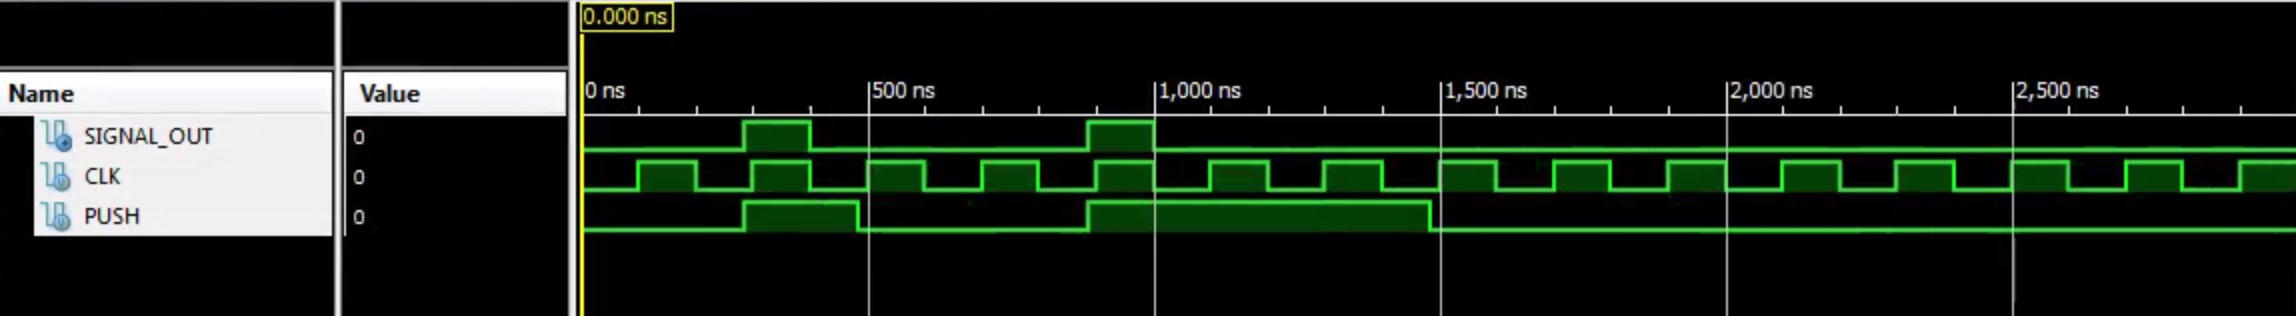
\includegraphics[scale=.4]{signal.PNG}\\
		\end{center}

		In this testbench you can see the clock signal schematic passes through one clock signal from the actual clock to signal out when the button attached to the PUSH variable is pushed. Note that you can see from the second push that it does not matter how long you push or hold the button attached to PUSH, one push will always pass one rising and fall clock edge not matter the hold time.

	\subsection{Bypass Clock Signal Testbench}
		\begin{center}
			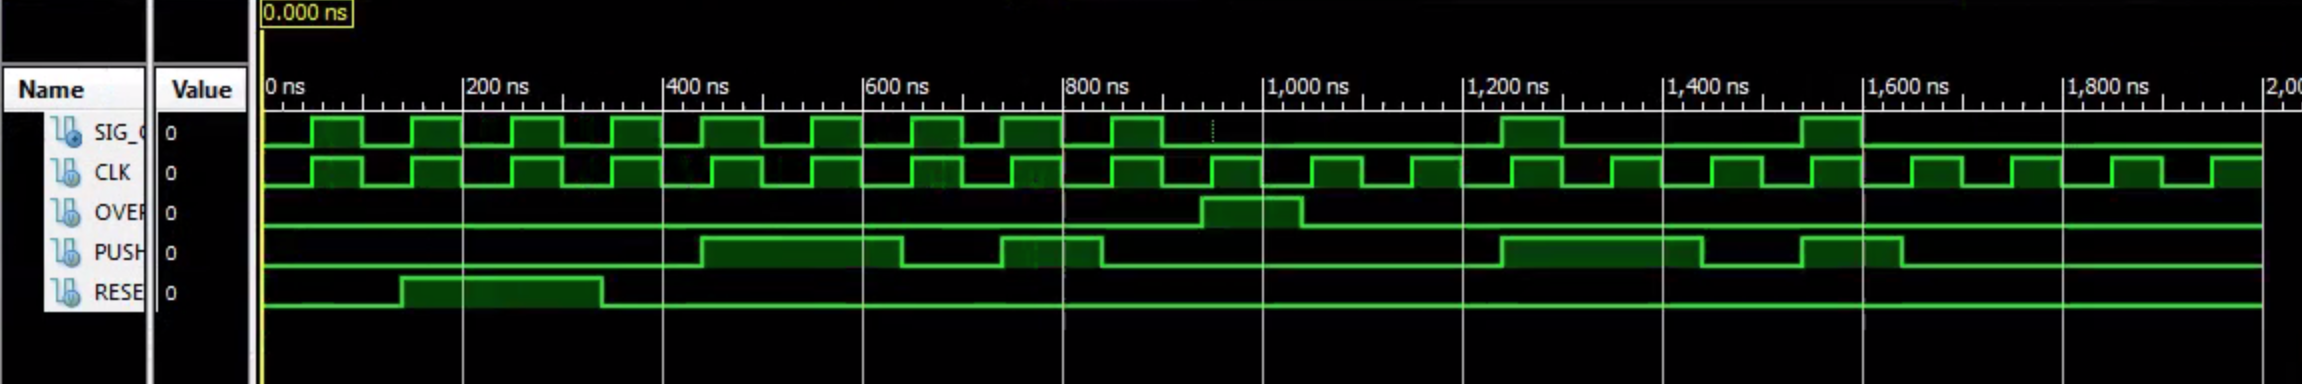
\includegraphics[scale=.4]{bypass.PNG}\\
		\end{center}

		This testbench demostrates the Bypass Clock Signal and is built off of Clock Signal tested above. This is supposed to combine the need to write all of ROM to RAM at the beginning of the program and the need to have a button pass through just one clock edge. Notice that on a RESET the Signal Out mirrors the actual clock signal until OVERFLOW goes high. This is because we need the signal out to mirror the clock to continually copy ROM to RAM without pushing any button. Moreover notice that before OVERFLOW goes high it doesnt matter how hard long or often you push the button attached to PUSH nothing happens. After OVERFLOW goes high everything acts exactly as it did in the clock signal testbench unless you hit RESET starting the whole process over again.

	\subsection{Running the Toy Processor on the BASys Board}
		The third portion of the demonstration was putting everything together, writting a UCF file, program ROM, and put it all on the board to run and test the whole processor. For the demo we ran a simple counter from 0 - 9 the logical way and a needlessly complicated way. The exact processes are explained above. The board operated entirely as expected.
	
	\newpage
\section{Significance} \vspace{-.7cm} \line(1,0){470}
	\paragraph{} 
		This is what we have been working towards all semester. We have completed the memory ROM and RAM logic and practiced writing a program in ROM and testbenching everything put together. Finally we needed to manage having the ROM actually write its entire contents to RAM and have a button operate the pass through of the clock. Now we can write any program using the basic instructions we have encoded as long as it fits in memory. We have finally completed our own very very very simple processor.

 \section{Comments/Suggestions}\vspace{-.7cm} \line(1,0){470}
 	\paragraph{} 
 		The programming requirement counting from 0 - 9 in such a conviluted way as to use all the instructions is understandable but is far to complicated. You should either come up with an program that uses all the instructions more naturally or makes more sense or have each group write any of there own useful program so long as it uses all instructions.
		
\end{document}


